\documentclass[a4paper,10pt]{ctexart}
\usepackage[margin=1in]{geometry}

%\usepackage{aicescover} %使用新的封面

%\usepackage{titletoc} %使用此包目录生成Bug
\usepackage{abstract}
\usepackage{graphics}
\usepackage{amsmath}
\usepackage{amsfonts}
\usepackage{amssymb}
\usepackage{amsthm}

\usepackage{cite}

\usepackage[colorlinks,linkcolor=black,anchorcolor=blue,citecolor=green]{hyperref}

\usepackage{clrscode3e} %插入伪代码

\usepackage{listings} %插入C代码
\usepackage{xcolor}
\lstset{
    %行号
    numbers=left,
    %背景框
    framexleftmargin=10mm,
    frame=none,
    %背景色
    %backgroundcolor=\color[rgb]{1,1,0.76},
    backgroundcolor=\color[RGB]{245,245,244},
    %样式
    keywordstyle=\bf\color{blue},
    identifierstyle=\bf,
    numberstyle=\color[RGB]{0,192,192},
    commentstyle=\it\color[RGB]{0,96,96},
    stringstyle=\rmfamily\slshape\color[RGB]{128,0,0},
    %显示空格
    showstringspaces=false
}

\ctexset{section={
    name={第,章},
    number=\arabic{section},
    }
}

%\title{集合论实验报告:最短路径}
%\author{冯云龙
%\address{Harbin Institute of Technology}
%\email{15939423778@163.com}
%}

\begin{document}
%\maketitle
\begin{titlepage}

\begin{center}


% Upper part of the page

\includegraphics[width=0.8\textwidth]{./HIT.eps}\\[1cm]

\textsc{\LARGE Harbin Institute of Technology}\\[1.5cm]

% Title
\hrulefill \\[0.4cm]
{ \huge \bfseries 集合论实验报告:最短路径}\\[0.4cm]
\hrulefill \\[1.5cm]

% Author and supervisor
\begin{minipage}{0.4\textwidth}
\begin{flushleft} \large
%悬空
\end{flushleft}
\end{minipage}
\begin{minipage}{0.4\textwidth}
\begin{flushright} \large
\emph{作者:}冯云龙 \\
\emph{学号:}1160300202
\end{flushright}
\end{minipage}

\vfill

% Bottom of the page
{\large \today}

\end{center}
\end{titlepage}

\part*{摘要}
生活中的许许多多看似不同的问题在本质上却是相同的,我们对于问题的关注的也往往都是最省时,最省钱...这个时候,通过对图论问题的研究,我们就可以对这些问题做出解答,此报告主要回答关于图论中最短路径的问题。
\\
\tableofcontents

\newpage
\part{正文}
\section{实验背景}

\subsection{实验目的}
在实际生活中,我们常常会遇到关注点在于最短、最近、最省钱这些方面的问题,就比如下列问题:
\begin{itemize}
\item 一批货从北京到武汉的的最快,或最省钱的走法。
\item 在城市群中建一个仓储基地,建在什么位置可以让各个城市的送货速度都比较快。
\end{itemize}
而像这样的问题,我们都可以通过将其转化为图的问题来解决。

\subsection{实验方法}
诸如以上问题,我们都可以通过将其转化成图,而后使用求解图的方法解决它。
例如,上述一个和距离有关的问题,我们就可以将其按如下方式转化:
取图$G(V,E,W)$,城市所对应的顶点集$(V_0,V_1...V_{n-1}) \in V $,若两个城市$V_i,V_j$邻接,距离为$w$,则有$(V_i,V_j)\in E$,$W(V_i,V_j)=w$。

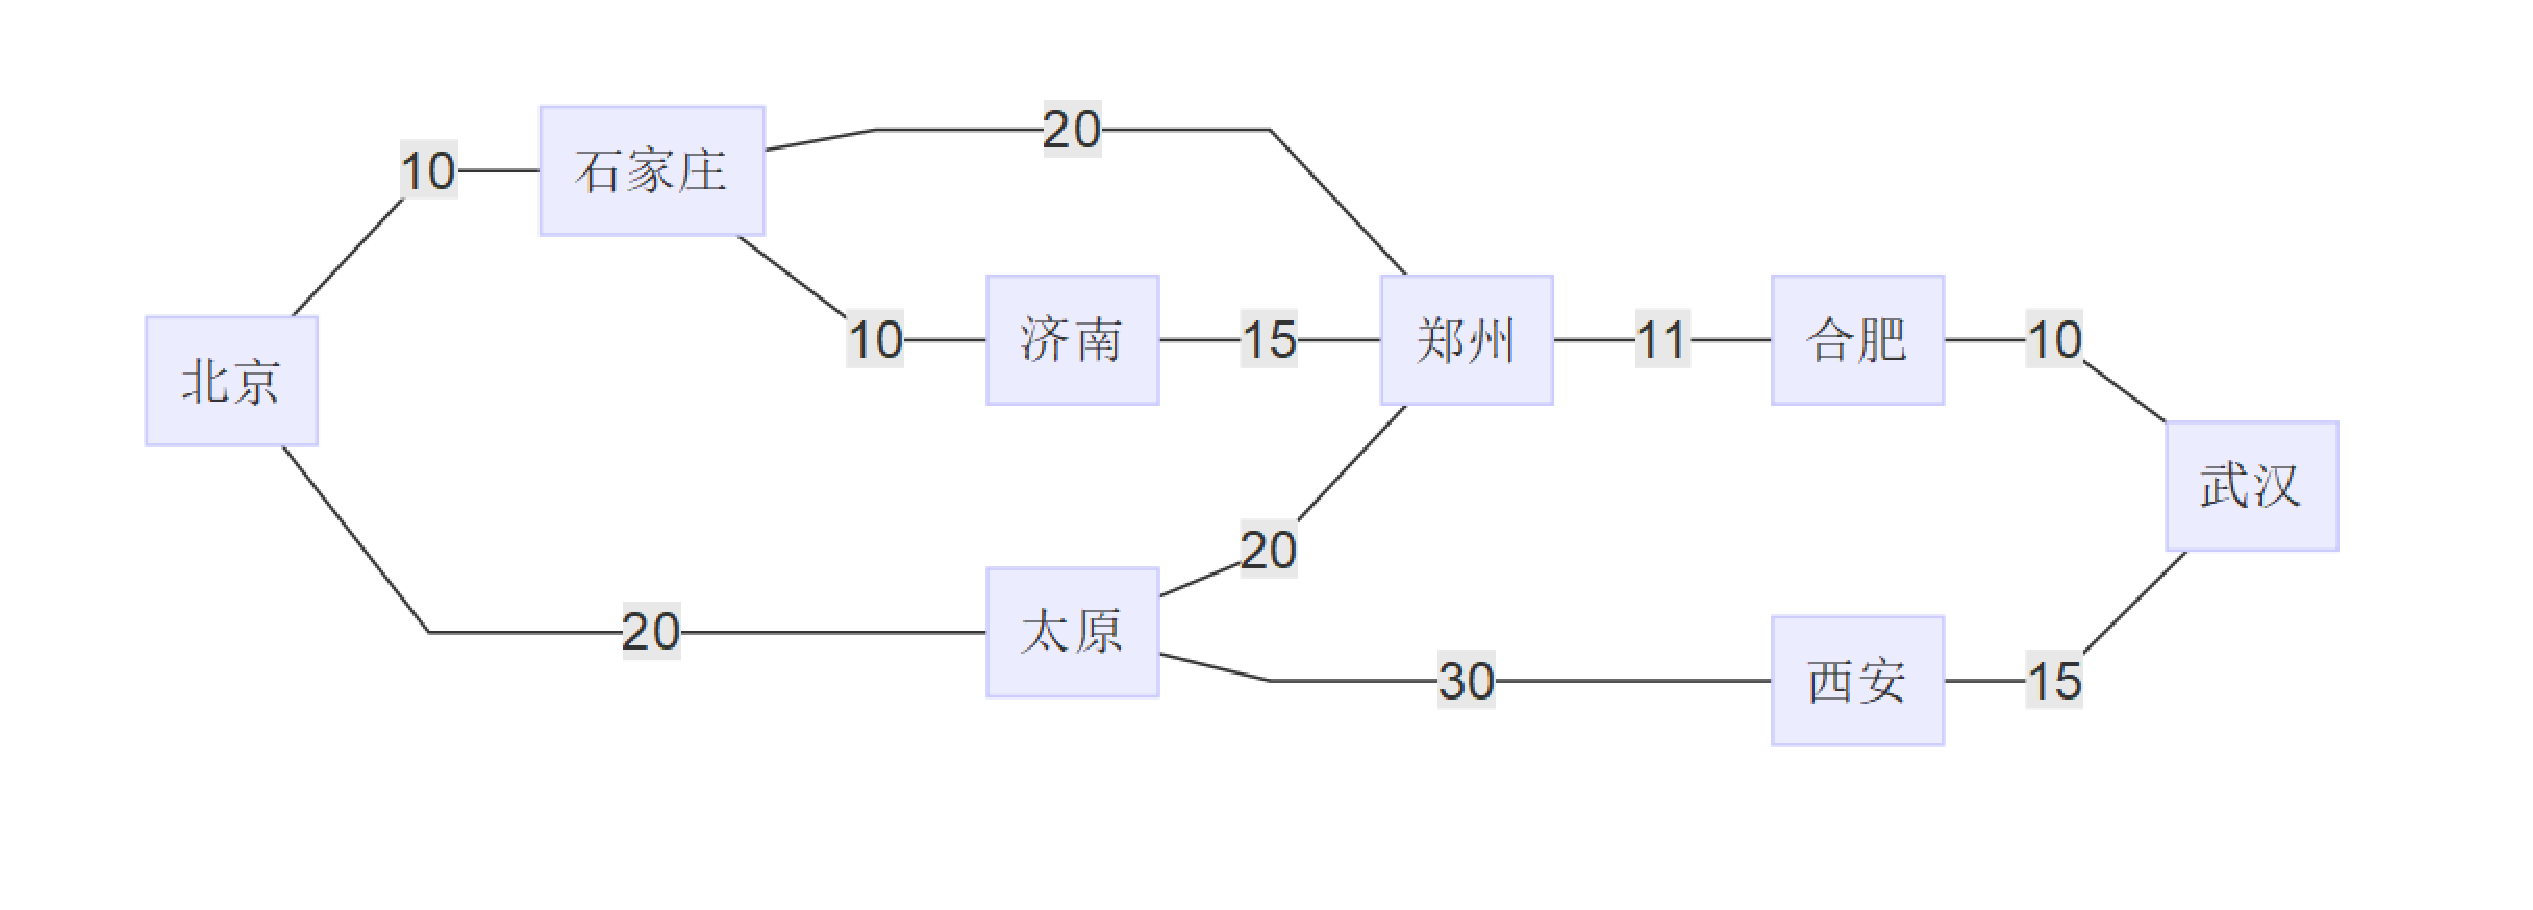
\includegraphics[width=0.9\textwidth]{MiniLen.eps}

\section{实验原理}
\subsection{迪杰斯特拉算法思想}
\begin{itemize}
\item 设$G=(V,E,W)$是一个带权有向图,把图中顶点集合$V$分成两组:
    \begin{enumerate}
    \item 第一组为已求出最短路径的顶点集合(用$S$表示)
    \item 第二组为其余未确定最短路径的顶点集合(用$U$表示)
    \end{enumerate}
\item 初始时$S$中只有一个源点,以后每求得一条最短路径 , 就将加入到集合$S$中,直到全部顶点都加入到$S$中,算法就结束了。
\item 按最短路径长度的递增次序依次把第二组的顶点加入$S$中。在加入的过程中,总保持从源点$v$到$S$中各顶点的最短路径长度不大于从源点$v$到$U$中任何顶点的最短路径长度。
\item 此外,每个顶点对应一个距离,$S$中的顶点的距离就是从$v$到此顶点的最短路径长度,$U$中的顶点的距离,是从$v$到此顶点只包括$S$中的顶点为中间顶点的当前最短路径长度。
\end{itemize}
\subsection{迪杰斯特拉算法步骤}
\begin{enumerate}
  \item 初始时,$S$只包含源点,即$S={v}$,$v-v$的距离为0。$U$包含除$v$外的其他顶点,即:$U=V \setminus S$,若$v$与$U$中顶点$u$有边,则$<u,v>$正常有权值,若u不是$v$的出边邻接点,则$<u,v>$权值为$ \infty $。
  \item 从$U$中选取一个距离$v$最小的顶点$k$,把$k$,加入$S$中(该选定的距离就是$v$到$k$的最短路径长度)。
  \item 以$k$为新考虑的中间点,修改$U$中各顶点的距离;若从源点$v$到顶点$u$的距离(经过顶点$k$)比原来距离(不经过顶点$k$)短,则修改顶点u的距离值,修改后的距离值的顶点k的距离加上边上的权。
  \item 重复步骤2和3直到所有顶点都包含在$S$中。
\end{enumerate}

\section{代码实现}
\subsection{设计数据结构}
参照了耶鲁大学的一位前辈的代码,动态分配数组,长度可以扩展,既不浪费空间,有不会带来性能损失。
数据结构如下\ref{数据结构如下}:


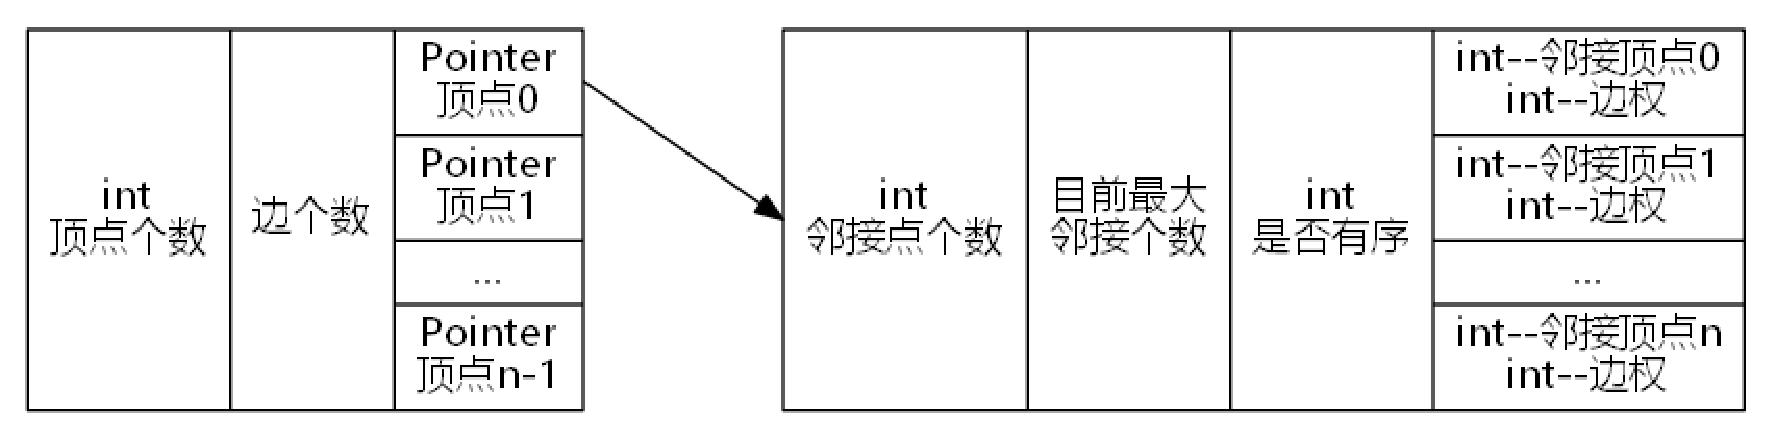
\includegraphics[width=0.9\textwidth]{DataStruct.eps}

\subsection{设计数据操作}
\begin{enumerate}
  \item 创建一个顶点从$0 \to n-1$的带权图
  \item 从内存中删去一个图
  \item 添加边和权
  \item 返回顶点个数
  \item 返回边个数
  \item 返回顶点的度
  \item 判断是否邻接
  \item 获取边的权
  \item 提供读取顶点数据的接口
\end{enumerate}

\subsection{实现迪杰斯特拉算法}
\begin{itemize}
  \item 定义数据结构
  \item 迪杰斯特拉算法实现\ref{最短路径实现}
\end{itemize}
\begin{codebox}
\Procname{$\proc{Dijkstra's Algorithm}(G,v_0)$}
\li \For $v \in \attrib{G}{V}$
    \Do
\li     $Dis(v) \gets \attrib{G}{W}(v,v_0)$
    \End
\li $Set \  v_0 \in S$
\li \While $S \ne \attrib{G}{V}$
    \Do
\li     $k \gets \attrib{Dis(V)}{V_m}$
\li     $Set \  k \in S$
\li     \For $v \notin S$
        \Do
\li        \If $Dis(k) + \attrib{G}{W}(k,v) < Dis(v)$
\li        \Then $Dis(v) \gets Dis(k) + \attrib{G}{W}(k,v)$
\li        $Prev(v) = k $
        \End
    \End
\end{codebox}
\section{实验结果}
\subsection{数据输入}
输入如下无向带权图\\
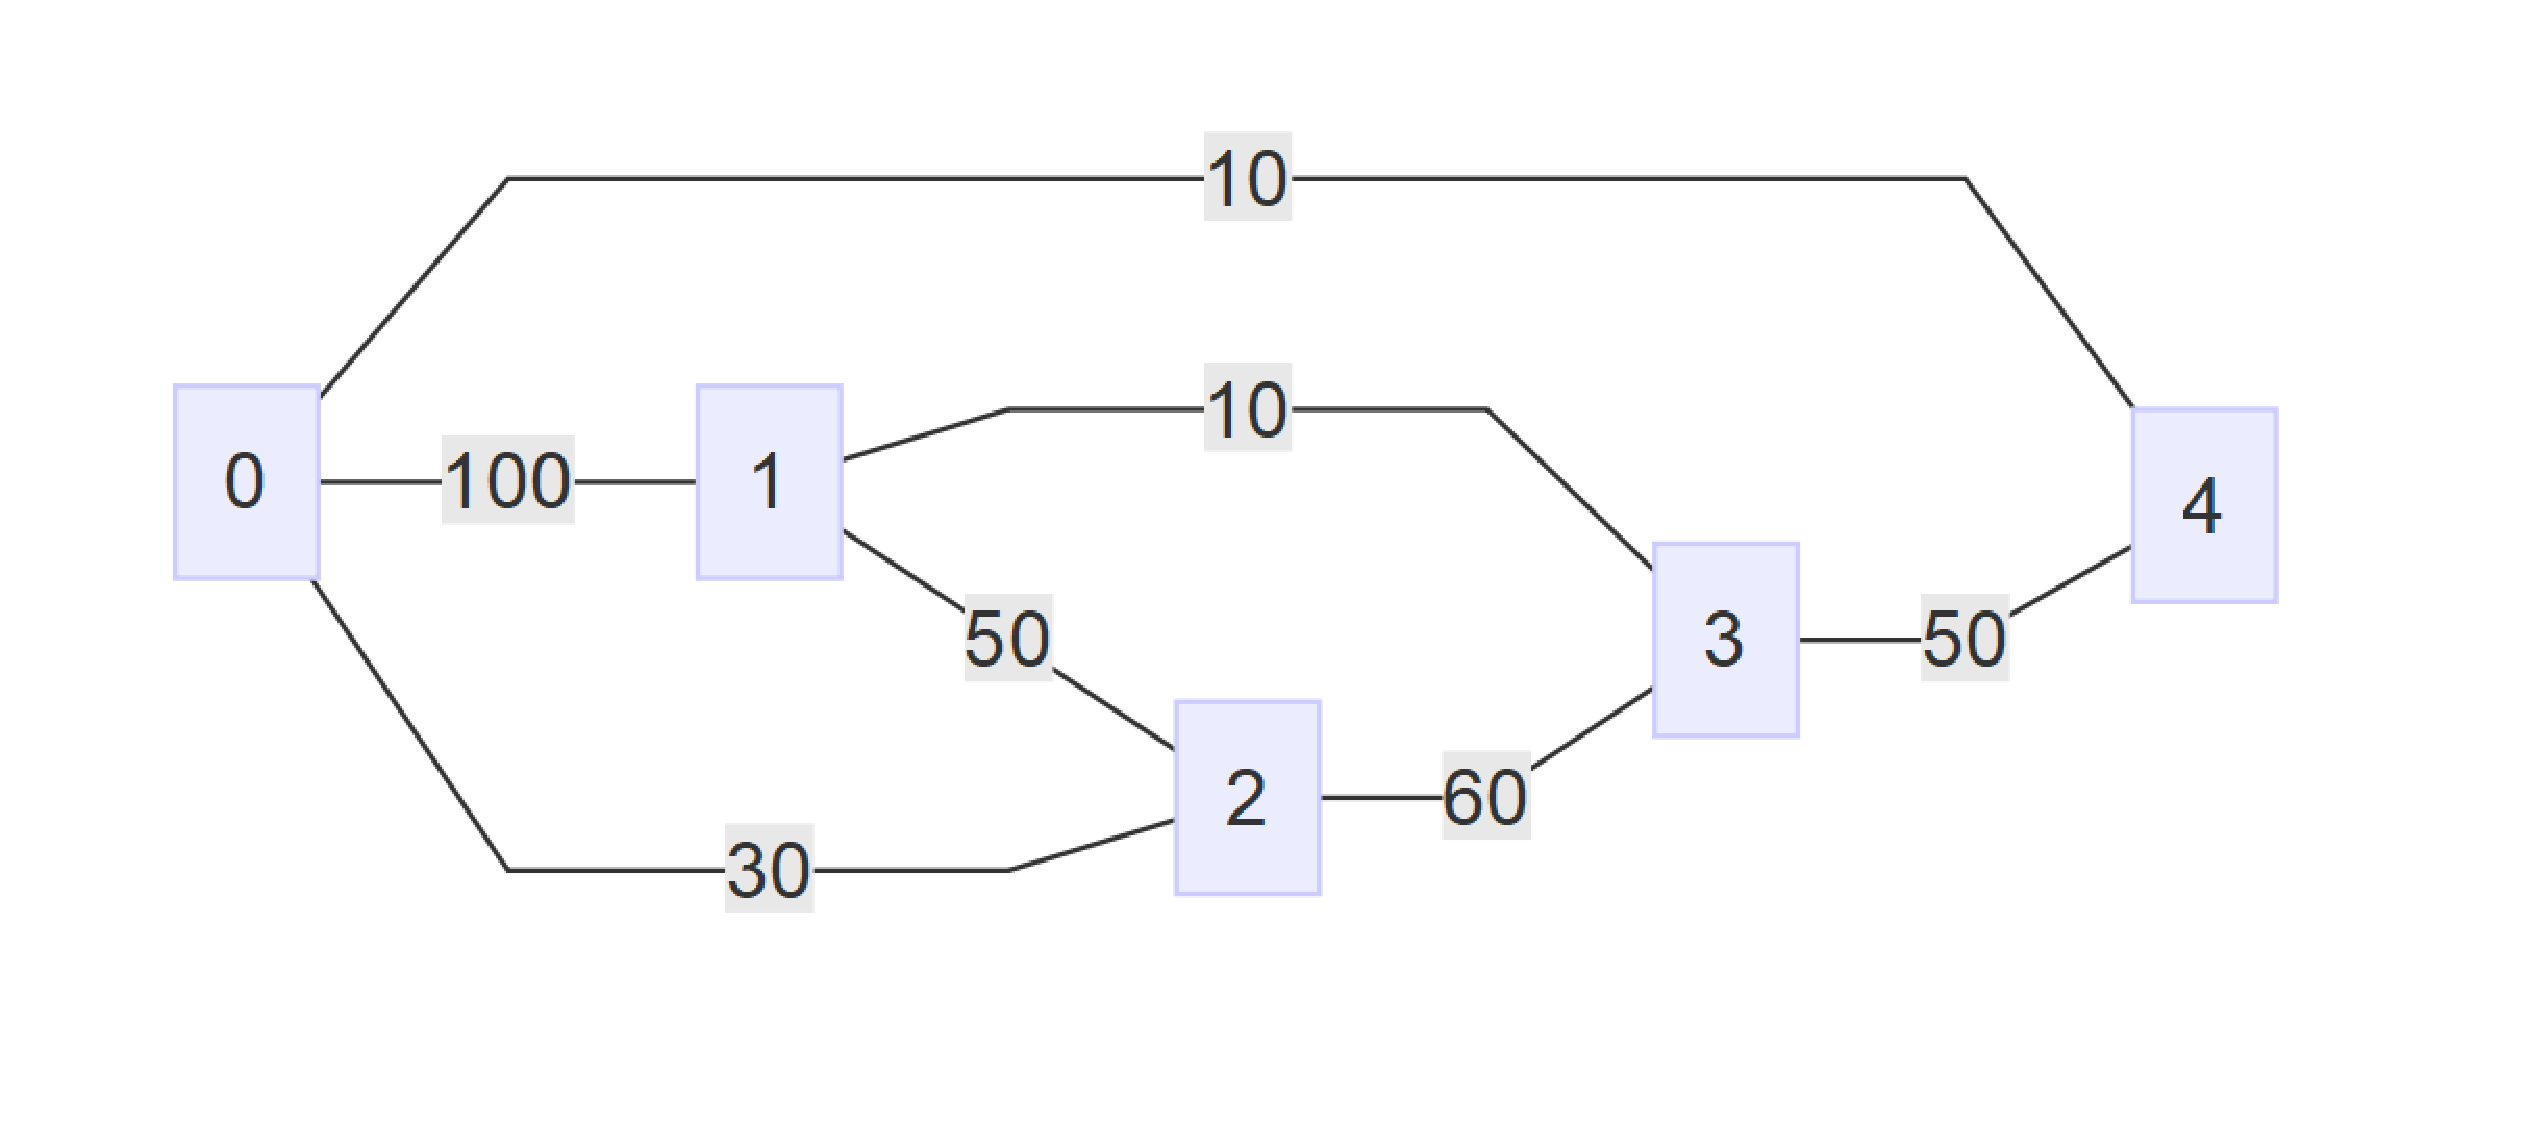
\includegraphics[width=0.9\textwidth]{Test.eps}
\subsection{结果输出}
通过迪杰斯特拉算法可得到如下结果,既得出距离,又可以显示路径\\
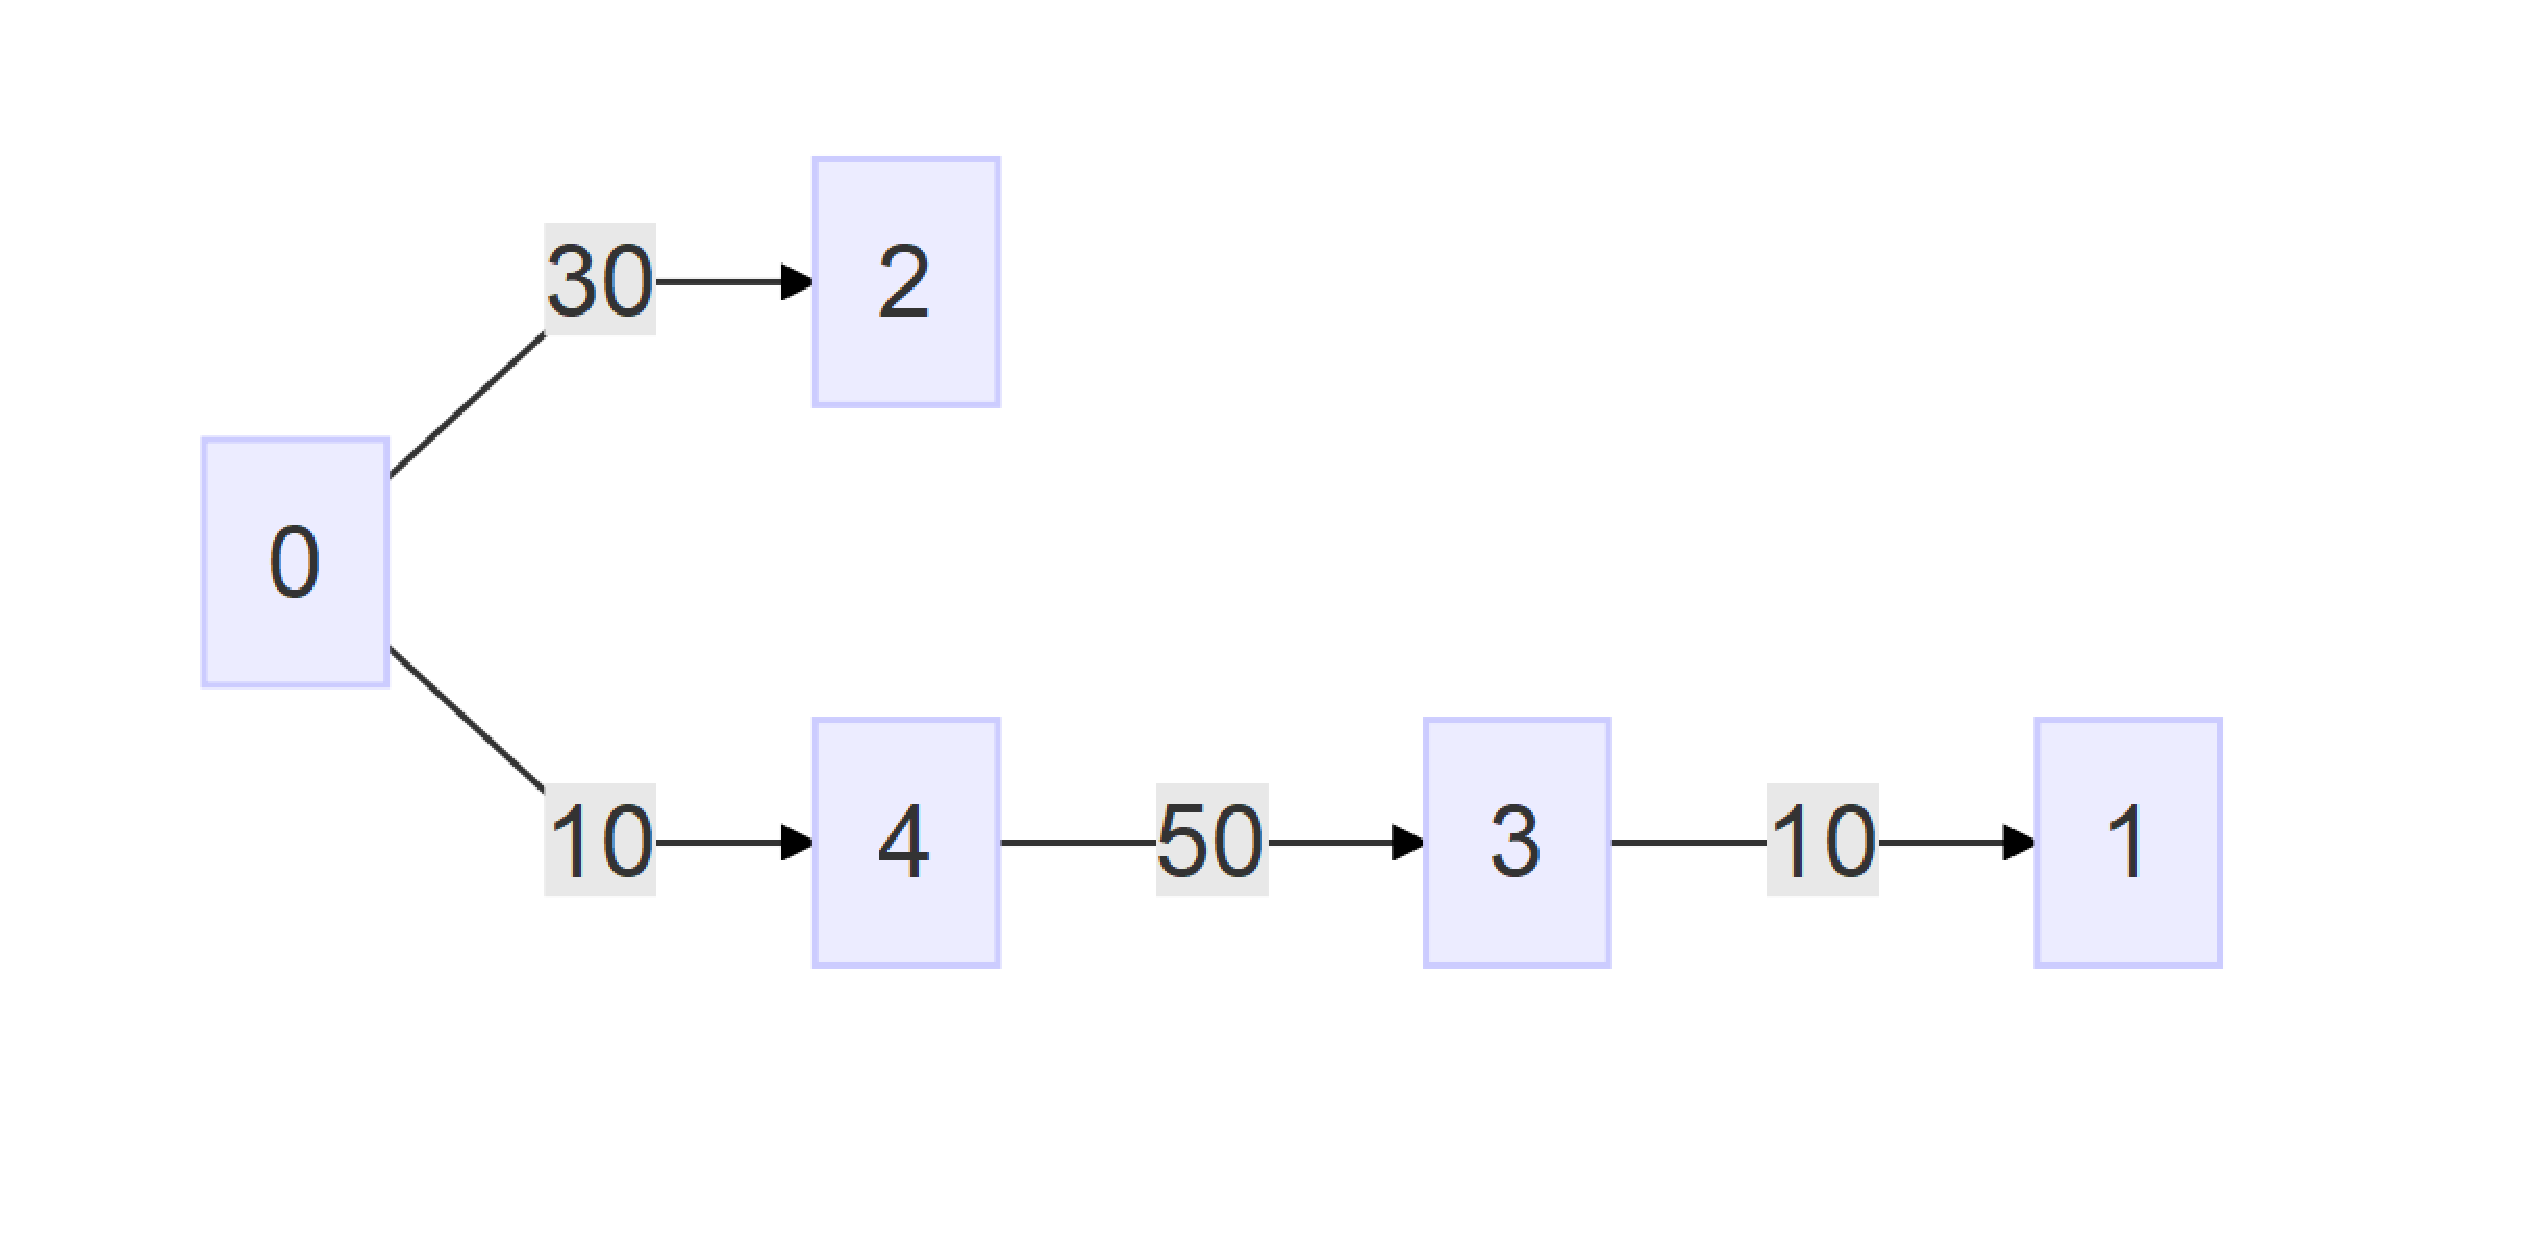
\includegraphics[width=0.9\textwidth]{Test-MinLen.eps}

\section{实验分析}
\subsection{效率分析}
迪杰斯特拉算法的时间复杂度是$O(n^2)$,空间复杂度则取决于数据结构,使用矩阵则为$O(n^2)$。
\subsection{同类算法比较}
相对于弗洛伊德算法迪杰斯特拉算法来说,迪杰斯特拉算法不能能处理边权为负值的情况。
\subsection{优化策略}
\paragraph{权值排序优化策略}
将要扫描的结点按其对应弧的权值进行顺序排列,每循环一次即可得到符合条件的结点,大大提高了算法的执行效率。
\paragraph{A*算法优化策略}
采用改进的Dijkstra算法——A*算法。A*算法是人工智能运用在游戏中的一个重要实践,它主要是解决路径搜索问题。A*算法实际是一种启发式搜索。所谓启发式搜索,就是利用一个估价函数judge()评估每次决策的价值,决定先尝试哪一种方案。这样可以极大地优化普通的广度优先搜索。从Dijkstra算法到A*算法是判断准则的引入,如果这个判断条件不成立,同样地,只能采用Dijkstra算法。所以A*算法中的估价函数是至关重要。
\paragraph{扇形优化策略}
从尽量减少最短路径分析过程中搜索的临时结点数量,限制范围搜索和限定方向搜索考虑进行优化。那么这种有损算法是否可行呢?我们知道,现实生活中行进,不会向着目的地的相反方向行进,否则就是南辕北辙。所以,当所研究的网络可以抽象化为平面网络的条件下,也不必搜索全部结点,可以在以源点到终点所在直线为轴线的扇形区域内搜索最短路径。这样,搜索方向明显地趋向终点,提高了搜索速度,虽然抛弃了部分结点,但基本上不影响搜索的成功率。

\newpage
\appendix
\part{附录}
\section{带权图实现}
\label{数据结构如下}
\begin{lstlisting}[language={C}]
//
// Created by Along on 2017/5/13.
//

#include <stdlib.h>
#include <assert.h>

#include "WeightGraph.h"

//基础带权图定义
//使用可变数组表示的临接矩阵


typedef struct _list {
    int vec;            //临接顶点
    int weight;         //权
} link_list;

struct w_graph {
    int n;                      //顶点个数
    int m;                      //边个数
    struct successors {
        int d;                  //临接点个数
        int len;                //最大临接点个数
        char is_sorted;         //
        link_list list[1];              //临接列表
    } *v_list[1];
};


//创建一个顶点从0 ~ n-1的带权图
WGraph w_graph_create(int n) {
    WGraph g;
    int i;

    g = malloc(sizeof(struct w_graph) +
    sizeof(struct successors *) * (n - 1));
    assert(g);

    g->n = n;
    g->m = 0;

    for (i = 0; i != n; i++) {
        g->v_list[i] = malloc(sizeof(struct successors));
        assert(g->v_list[i]);
        g->v_list[i]->d = 0;
        g->v_list[i]->len = 1;
        g->v_list[i]->is_sorted = 1;
    }

    return g;
}

//释放内存
void w_graph_destroy(WGraph g) {
    int i;

    for (i = 0; i != g->n; i++) {
        free(g->v_list[i]);
    };
    free(g);
}

//添加边和权
void w_graph_add_edge(WGraph g, int u, int v, int weight) {
    assert(u >= 0);
    assert(u < g->n);
    assert(v >= 0);
    assert(v < g->n);

    //是否需要增长list
    while (g->v_list[u]->d >= g->v_list[u]->len) {
        g->v_list[u]->len *= 2;
        g->v_list[u] =
                realloc(g->v_list[u], sizeof(struct successors) +
                 sizeof(link_list) * (g->v_list[u]->len - 1));
    }

    //添加新临接点
    g->v_list[u]->list[g->v_list[u]->d].vec = v;
    g->v_list[u]->list[g->v_list[u]->d].weight = weight;

    g->v_list[u]->d++;

    g->v_list[u]->is_sorted = 0;

    //边数+1
    g->m++;
}

//返回顶点个数
int w_graph_vector_count(WGraph g) {
    return g->n;
}

//返回边个数
int w_graph_edge_count(WGraph g) {
    return g->m;
}

//返回顶点的度
int w_graph_out_degree(WGraph g, int source) {
    assert(source >= 0);
    assert(source < g->n);

    return g->v_list[source]->d;
}

//是否需要进行二分搜索和排序
#define BSEARCH_THRESHOLD (10)

static int list_cmp(const void *a, const void *b) {
    return ((const link_list *) a)->
    vec - ((const link_list *) b)->vec;
}


#include <stdio.h>

//二者之间有边则返回1
int w_graph_has_edge(WGraph g, int source, int sink) {
    int i;

    assert(source >= 0);
    assert(source < g->n);
    assert(sink >= 0);
    assert(sink < g->n);

    if (w_graph_out_degree(g, source) >= BSEARCH_THRESHOLD) {
        //确保已经被排序
        if (!g->v_list[source]->is_sorted) {
            qsort(g->v_list[source]->list,
                  g->v_list[source]->d,
                  sizeof(link_list),
                  list_cmp);
        }
        //使用二分查找
        link_list to_find;
        to_find.vec = sink;
        to_find.weight = 0;

        return bsearch(&to_find,
                       g->v_list[source]->list,
                       g->v_list[source]->d,
                       sizeof(link_list),
                       list_cmp) != 0;
    } else {
        //数据量很少,直接遍历
        int vec_degree = g->v_list[source]->d;
        for (i = 0; i != vec_degree; i++) {
            if (g->v_list[source]->list[i].vec == sink) {
                return 1;
            }
        }
    }
    return 0;
}

//返回权
int w_graph_weight_edge(WGraph g, int source, int sink) {
    int i;

    assert(source >= 0);
    assert(source < g->n);
    assert(sink >= 0);
    assert(sink < g->n);

    if (w_graph_out_degree(g, source) >= BSEARCH_THRESHOLD) {
        //确保已经被排序
        if (!g->v_list[source]->is_sorted) {
            qsort(g->v_list[source]->list,
                  g->v_list[source]->d,
                  sizeof(link_list),
                  list_cmp);
        }
        //使用二分查找
        link_list to_find;
        to_find.vec = sink;
        to_find.weight = 0;
        link_list *res = bsearch(&to_find,
                                 g->v_list[source]->list,
                                 g->v_list[source]->d,
                                 sizeof(link_list),
                                 list_cmp);
        return res->weight;
    } else {
        //数据量很少,直接遍历
        for (i = 0; i != g->v_list[source]->d; i++) {
            if (g->v_list[source]->list[i].vec == sink) {
                int res = g->v_list[source]->list[i].weight;
                return res;
            }
        }
        return INFINITY;
    }
}

//提供数据 遍历接口
void w_graph_foreach(WGraph g, int source,
void (*f)(WGraph, int, int, int, void *), void *data) {
    int i;

    assert(source >= 0);
    assert(source < g->n);

    for (i = 0; i != g->v_list[source]->d; ++i) {
        f(g, source, g->v_list[source]->list[i].vec,
         g->v_list[source]->list[i].weight, data);
    }
}
\end{lstlisting}
\section{最短路径实现}
\label{最短路径实现}
\begin{lstlisting}[language={C}]
//
// Created by Along on 2017/5/13.
//

#include <stddef.h>
#include <assert.h>
#include <malloc.h>
#include <stdio.h>
#include "WeightGraph.h"
#include "Graph_tools.h"

struct min_len {
    int n;
    int vec;
    struct list {
        int dist;           //与所要求顶点的距离
        int prev;           //前驱动点
    } a_list[1];
};

//迪杰斯特拉算法
Min_len Dijkstra(WGraph g, int source) {
    int i, j, *S;
    Min_len res;

    int vec_num = w_graph_vector_count(g);

    assert(source >= 0);
    assert(source < vec_num);

    res = malloc(sizeof(struct min_len) +
    sizeof(struct list) * (vec_num - 1));
    S = calloc((size_t) vec_num, sizeof(int));
    assert(res);
    assert(S);

    res->n = vec_num;
    res->vec = source;

    //初始化各点
    for (i = 0; i != vec_num; ++i) {
        S[i] = 0;
        if (w_graph_has_edge(g, source, i)) {
            res->a_list[i].dist = w_graph_weight_edge(g, source, i);
            res->a_list[i].prev = source;
        } else {
            res->a_list[i].prev = -1;
            res->a_list[i].dist = INFINITY;
        }
    }

    res->a_list[source].dist = 0;
    res->a_list[source].prev = source;
    S[source] = 1;

    for (i = 1; i != vec_num; ++i) {
        int min_dst = INFINITY;
        int u = source;
        //找出未使用过的点中dist最小的
        for (j = 0; j != vec_num; ++j) {
            if ((!S[j]) && res->a_list[j].dist < min_dst) {
                u = j;     //u是距离source最近的点
                min_dst = res->a_list[j].dist;
            }
        }

        S[u] = 1;    //将u标记为已使用

        for (j = 0; j != vec_num; ++j)
        //j点未被使用且u,j之间有边
            if ((!S[j]) && w_graph_has_edge(g, u, j)) {
                if (res->a_list[u].dist + w_graph_weight_edge(g, u, j)
                 < res->a_list[j].dist) {
                    res->a_list[j].dist = res->a_list[u].dist +
                    w_graph_weight_edge(g, u, j);   //更新距离
                    res->a_list[j].prev = u;        //更新路径
                }
            }
    }
    free(S);
    return res;
}

//数据遍历接口
void min_len_foreach(Min_len m,
void (*f)(Min_len, int, int, void *), void *data) {
    int i;
    for (i = 0; i != m->n; i++) {
        f(m, m->a_list[i].dist, m->a_list[i].prev, data);
    }
}

//顶点个数
int min_len_vector_count(Min_len m) {
    return m->n;
}

//释放内存
void min_len_destroy(Min_len m) {
    free(m);
}

//封装一次添加二条边
void w_graph_add_edge2(WGraph g, int source, int sink, int weight) {
    w_graph_add_edge(g, source, sink, weight);
    w_graph_add_edge(g, sink, source, weight);
}

//打印数据
static void w_graph_show_vec(WGraph g, int src, int sink,
int weight, void *data) {
    printf(" %d:%d ", sink, weight);
}

//调用接口
void min_len_show(Min_len ml) {
    int i, j;
    for (i = 0; i != ml->n; ++i) {
        printf("Dist:%d ", ml->a_list[i].dist);
        for (j = i; j != ml->vec; j = ml->a_list[j].prev) {
            printf("%d <- ", j);
        }
        printf("%d\n", ml->vec);
    }
}
\end{lstlisting}
\end{document} 